\subsection{Wiring a Generic Small World Graph} \label{sec:proof1}

Consider a set of computational nodes arranged in an $r$-dimensional mesh.
In each dimension, physical interconnects run between immediately adjacent pairs of nodes.
Represent this physical hardware with a graph $N$.
Vertices of $N$, $V(N)$, represent computational nodes.
Edges of $N$, $E(N)$, represent physical interconnects between nodes.

Let $d(a,b)$ represent the typical number of physical interconnects traversed on a shortest path between a pair of arbitrary nodes $a, b \in V(N)$.
This is conceptually equivalent to Manhattan distance.

In the case of a one-dimensional sequence of nodes, for a pair of arbitrary nodes $a,b \in V(N)$,
\begin{align*}
\bar{d}(a,b) \propto |V(N)|.
\end{align*}

Consider next the case of a higher-dimensional grid topology, like a two-dimensional grid or a three-dimensional mesh.
Because $d$ is a Manhattan metric, the number of physical interconnects requiring traversal in each dimension on a shortest-path between two nodes is completely independent.

Arranging the set of nodes $N$ in a $r$-dimensional cube, cube width in each dimensions scales proportionally to the $r$-th root of $|V(N)|$.

So, for a pair of arbitrary nodes $a,b \in V(N)$,
\begin{align} \label{eqn:mesh_prop}
\bar{d}(a, b) \propto |V(N)|^{\frac{1}{r}} \times r
\end{align}

We proceed to construct a small world directed graph $G$ using the set of nodes $N$ as vertices.
In formal terms, a bijective relationship $f: V(N) \rightarrow V(G)$ unites these two sets.
The inverse mapping, $f^{-1}: V(G) \rightarrow V(N)$, is also bijective.

\begin{figure}[t]
\begin{center}
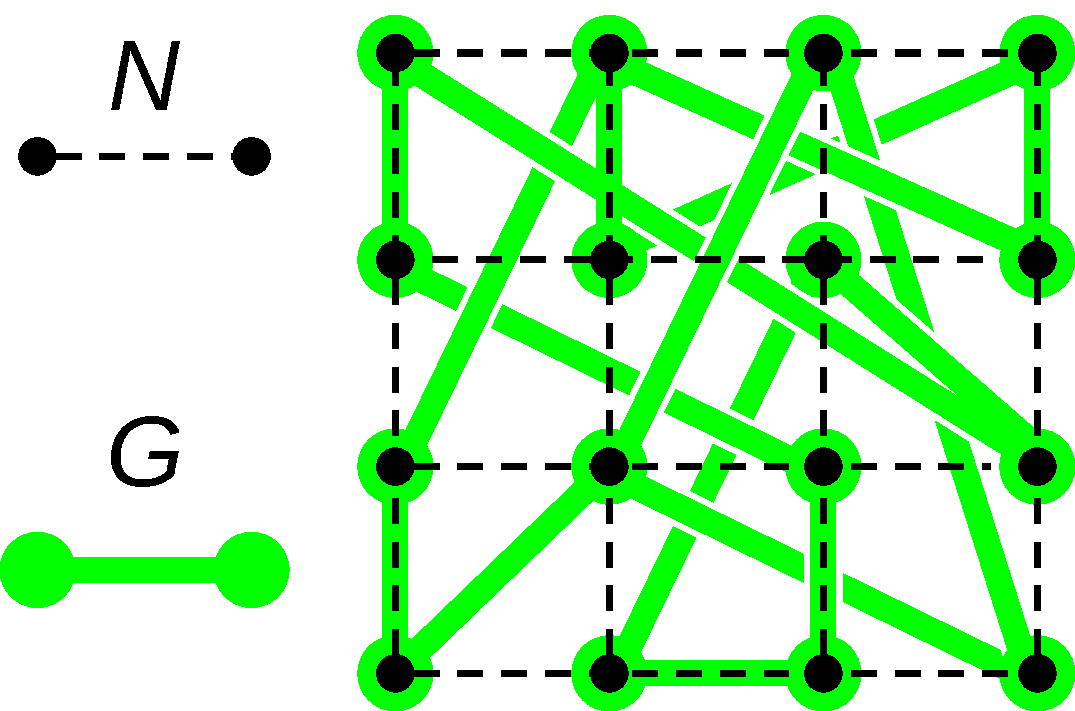
\includegraphics[width=\linewidth]{nandg}
\caption{
TODO
}
\label{fig:nandg}
\end{center}
\end{figure}


Edges in the graph $G$ do not represent a physical interconnect.
Instead, edges $\{\hat{a}, \hat{b}\} \in E(G)$ represent a close-coordination relationship where node $\hat{a}$ frequently interacts with (i.e., dispatches messages to) the destination node $\hat{b}$.
Figure \ref{fig:nandg} illustrates the relationship between $N$ and $G$.

Let $\hat{d}(\hat{a},\hat{b})$ denote distance between vertices $\hat{a}$ and $\hat{b}$ with respect to the graph $G$.
That is, the number of graph edges traversed on a shortest-path route between $\hat{a}$ and $\hat{b}$ over $G$.
In a small-world network, typical graph distance scales proportionally with the logarithm of network size \citep{watts1998collective}.
In our case, for arbitrary $\hat{a},\hat{b} \in V(G)$,
\begin{align} \label{eqn:smallworld_prop}
\bar{\hat{d}}(\hat{a},\hat{b}) \propto \log(|V(G)|).
\end{align}

Consider the sequence of edges in $G$ traversed on a shortest-path route $R_{\hat{a},\hat{b}}$ between $\hat{a}, \hat{b} \in V(G)$, $\{\{\hat{x}_1, \hat{y}_1\}, \{\hat{x}_2, \hat{y}_2\}, \ldots, \{\hat{x}_n, \hat{y}_n\} \}$.
Because $d$ represents a shortest-path traversal of the Manhattan network $N$,
\begin{align} \label{eqn:path_hops_inequality}
\sum_{\{\hat{x}, \hat{y}\} \in  R_{\hat{a},\hat{b}}}
\Big[ d\Big(f^{-1}(\hat{x}), f^{-1}(\hat{y})\Big) \Big]
\geq
d\Big(f^{-1}(\hat{a}), f^{-1}(\hat{b})\Big).
\end{align}
(Otherwise, we would have found a shorter path through $N$ between $f^{-1}(\hat{a})$ and $f^{-1}(\hat{b})$, violating the Manhattan metric's triangle inequality.)

Recall that $\hat{a},\hat{b}$ are sampled uniformly from $V(G)$.
So, $f^{-1}(\hat{a}),f^{-1}(\hat{b})$ are sampled uniformly from $V(N)$.
Thus, Equation \ref{eqn:mesh_prop} allows us to establish the following lower bound,
\begin{align*}
d\Big(f^{-1}(\hat{a}), f^{-1}(\hat{b})\Big)
&\in
\Omega \Big(
  |V(N)|^{\frac{1}{r}} \times r
\Big).
\end{align*}

It follows from Inequality \ref{eqn:path_hops_inequality} that
\begin{align*}
\sum_{\{\hat{x}, \hat{y}\} \in  R_{\hat{a},\hat{b}}}
\Big[ d\Big(f^{-1}(\hat{x}), f^{-1}(\hat{y})\Big) \Big]
&\in
\Omega \Big(
  |V(N)|^{\frac{1}{r}} \times r
\Big).
\end{align*}

Equation \ref{eqn:smallworld_prop} tells us that the mean number of edges in $R_{\hat{a}, \hat{b}}$ is proportional to $\log(|V(G)|)$.
So, letting $\bar{d}$ represent the mean case,
\begin{align*}
\log(|V(G)|) \times \bar{d}\Big(f^{-1}(\hat{x}), f^{-1}(\hat{y})\Big)
&\in
\Omega \Big(
  |V(N)|^{\frac{1}{r}} \times r
\Big).
\end{align*}

Rearranging and simplifying, we arrive at a lower bound of mean distance over the Manhattan network $N$ traversed for a connection in the interaction network $G$,
\begin{align*}
\bar{d}\Big(f^{-1}(\hat{x}), f^{-1}(\hat{y})\Big)
&\in
\Omega \Big(
  \frac{
    |V(N)|^{\frac{1}{r}} \times r
  }{
    \log(|V(N)|)
  }
\Big).
\end{align*}

Note that edges $\{\hat{x},\hat{y}\}$ are not sampled uniformly from $E(G)$.
Instead, their sampling is weighted by edge betweenness centrality.
\footnote{
Consider all pairings of nodes in a graph.
Now, construct a multiset of paths that, for each possible node pairing, contains the shortest path between those two nodes.
Edge betweenness is the fraction of the paths in this mulitset that passes through a particular edge \citep{Lu2013}.
}

% Edge betweenness is associated with connectivity: a edge that, upon removal, subdivides a graph into disconnected components of equal size exhibits maximum edge betweenness.
% To account for this non-uniform sampling, we must consider the most extreme possibles case in uneven edge betweenness centrality.
% This is the perfectly hierarchical case: there is one edge that can be cut that cleaves the graph in two, there are two edges that can be cut that cleave a quarter of the graph off, there are four edges that can be cut that cleave an eight of the graph off, etcetera.
%
% Arrange this graph as a binary tree.
%
% The sum betweenness of each layer of edges $L$ of the tree of size $n$ is given as
% \footnote{
% In the case of the binary tree, where all connections are rendered impossible by the removal of any of their edges, the edge betweenness is equivalent to the fraction of connections disrupted.
% This formula is derived in terms of the total number of connections in the graph, minus the remaining connections below a removed edge, minus the remaining connections above a removed edge.
% Layers $L$ count, zero-indexed, from the bottom.
% }
% \begin{align*}
% \frac{n}{2^{L+1}}
% \times
% \Big(&\\
%   &\frac{
%     n \times (n-1)
%   }{
%     n \times (n -1)
%   }\\
%   &-
%   \frac{
%     (2^{L+1} - 1) \times (2^{L+1} - 2)
%   }{
%     n \times (n -1)
%   }\\
%   &-
%   \frac{
%     (n - 2^{L+1} + 1) \times (n - 2^{L+1})
%   }{
%     n \times (n -1)
%   }\\
% &\Big).
% \end{align*}
%
% Taking the limit as $n \rightarrow \infty$, this simplifies to
% \begin{align*}
% \lim_{n \rightarrow \infty}
% 2
% -
% \frac{
%   2^{L+1}
% }{
%   n
% }
% .
% \end{align*}
%
% Recall that $L$ ranges between 0 and $\log_2 n - 1$, so
%
% \begin{align*}
% 1
% \leq
% \lim_{n \rightarrow \infty}
% 2
% -
% \frac{
%   2^{L+1}
% }{
%   n
% }
% \leq
% 2
% \end{align*}
%
% Thus, each layer of the binary tree has the same total betweenness weight sum.
% So, each layer's fraction of total betweenness weight is proportional to $1/\log(n)$.
%
% So, each edge's fraction of total betweenness weight is proportional to
% \begin{align*}
% \frac{2^{L+1}}{n} \times \frac{1}{\log(n)}.
% \end{align*}
%
% Recalling, again, that $0 \geq L \geq \log(n) - 1$, each edge's fraction of total betweenness weight is upper bounded by
% \begin{align*}
% \frac{1}{\log(n)}.
% \end{align*}
%
% and each edge's fraction of total betweenness weight is lower bounded by
% \begin{align*}
% \frac{1}{n \log(n)}.
% \end{align*}
%
% Physical distance over any edge $e \in G$ are upper bounded by
% \begin{align*}
% v_i \leq |V(N)|^{1/3}
% \end{align*}
%
% Let us write an expression for $C$ such that
% \begin{align*}
% \mu
% &=
% \mu_w \times C \\
% \sum \frac{1}{n} v_i
% &= C \times \sum \Big[ w_i \times v_i \Big] \\
% C
% &= \frac{
%   \frac{1}{n} \times \sum v_i
% }{
%   \sum \Big[ w_i \times v_i \Big]
% }
% \end{align*}
%
% Note that $\sum w_i = 1$.
%
% LOWER BOUND ON $C$ MEANS UPPER BOUND ON DENOMINATOR
% \begin{align*}
% C
% &\in \Omega\Big(\frac{
%   \frac{1}{n} \times \sum v_i
% }{
%   \sum_{\log n} \Big[ 1/(\log n) \times v_i \Big] + \sum_{n - \log n} \Big[ 1/(n \log n) \times v_i \Big]
% } \Big)\\
% C
% &\in \Omega\Big(\frac{
%   \frac{1}{n} \times \sum v_i
% }{
%   1/(\log n) \times \sum_{\log n} v_i + 1/(n \log n) \times \sum_{n - \log n}  v_i
% } \Big)\\
% &\in \Omega\Big(\frac{
%   \log n \sum v_i
% }{
%   n \times \sum_{\log n} v_i + \sum_{n - \log n}  v_i
% } \Big)\\
% &\in \Omega\Big(\frac{
%   \log n \sum v_i
% }{
%   (n-1) \times \sum_{\log n} v_i + \sum  v_i
% } \Big)\\
% &\in \Omega\Big(\frac{
%   \log n \sum v_i
% }{
%   (n-1) \times \log n \times n^{1/3} + \sum  v_i
% } \Big)\\
% &\in \Omega\Big(\frac{
%   1
% }{
%   \frac{(n-1) \times n^{1/3}}{\sum  v_i} + 1 / \log n
% } \Big)\\
% &\in \Omega\Big(\frac{
%   \sum  v_i
% }{
%   (n-1) \times n^{1/3}
% } \Big)\\
% &\in \Omega\Big(\frac{
%   \sum  v_i
% }{
%   n^{4/3}
% } \Big)\\
% &\in \Omega\Big(\frac{
%   \frac{1}{n} \sum  v_i
% }{
%   n^{1/3}
% } \Big)\\
% &\in \Omega\Big(\frac{
%   \mu
% }{
%   n^{1/3}
% } \Big)\\
% &\in \Omega\Big(\frac{
%   c
% }{
%   n^{1/3}
% } \Big)
% \end{align*}
%
% Hence, we attain a lower bound of the mean number of physical interconnects traversed for each connection sampled uniform interaction network $G$,
% \begin{align*}
% \bar{d}(x, y)
% &\in
% \Omega \Big(
%   \frac{|V(N)|^{\frac{1}{3}}}{\log(|V(N)|)} \times \frac{1}{|V(N)|^{1/3}}
% \Big)\\
% &\in
% \Omega \Big(
%   \frac{1}{\log(|V(N)|)}
% \Big).
% \end{align*}
%
%
% (log(n) \times n^{1/3} + (n - log(n)) \times c) / n
%
% log(n) \times n^{1/3} + (1 - log(n)/n)
%
% log(n)/n^{2/3} + (1 - log(n)/n)
%
% 1
